\subsection{Problem 1: Multi-layer Perceptron (MLP) and Feature Extraction on ReducedMNIST}

The objective of this problem is to classify the ReducedMNIST digits using MLP classifiers and compare them against classical machine learning models using different feature extraction methods. The dataset follows the assignment split of 1000 training images per digit and 200 testing images per digit.

\subsubsection{Part A: MLP Hyperparameter Tuning (Raw Pixels)}
Initially, the MLP architecture was tested on the raw pixel data to determine the optimal depth and regularization strategies. The hidden layers used ReLU activations, and the main configurations used Batch Normalization and Dropout. The Adam optimizer minimized categorical cross-entropy with an initial learning rate of $0.001$. Two extra diagnostic runs were also executed: one without regularization and one with a higher learning rate.

\begin{table}[H]
    \centering
    \caption{MLP Hyperparameter Tuning Results (Raw Pixels)}
    \label{tab:prob1_mlp_tuning}
    \resizebox{\linewidth}{!}{
    \begin{tabular}{|l|c|c|c|c|c|}
        \hline
        \textbf{Configuration} & \textbf{Hidden Layers} & \textbf{Regularization} & \textbf{Accuracy} & \textbf{Training Time} & \textbf{Testing Time} \\
        \hline
        Exp1: 1-hidden layer & 1 & Yes & 96.8\% & 7111.6 msec & 113.9 msec \\
        Exp2: 3-hidden layers & 3 & Yes & 97.3\% & 9993.0 msec & 121.9 msec \\
        Exp3: 4-hidden layers & 4 & Yes & 97.7\% & 11824.0 msec & 133.3 msec \\
        Exp4: 3-hidden, no regularization & 3 & No & 96.8\% & 5333.0 msec & 119.5 msec \\
        Exp5: 3-hidden, high learning rate & 3 & Yes & 97.2\% & 8338.0 msec & 124.3 msec \\
        \hline
    \end{tabular}
    }
\end{table}

\begin{figure}[H]
    \centering
    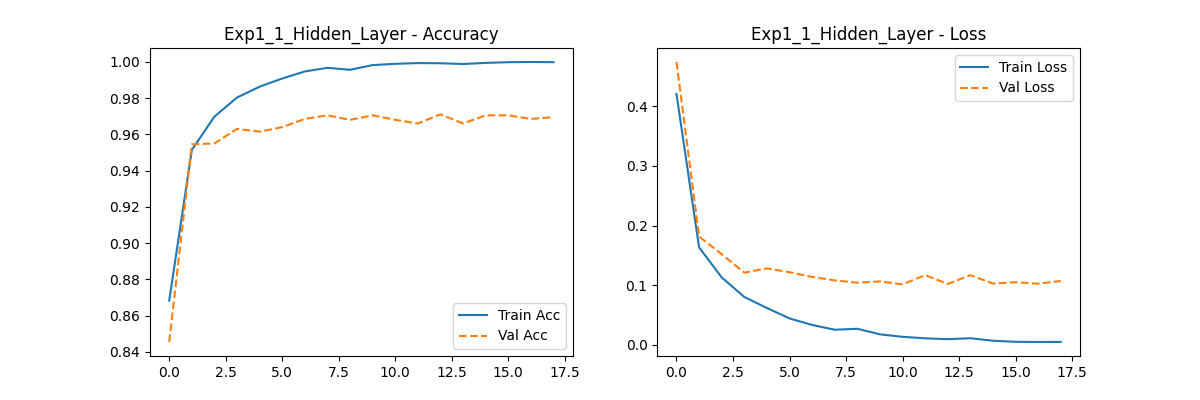
\includegraphics[width=0.75\linewidth]{../Part1_Problem1_MLP/results/Exp1_1_Hidden_Layer_Curves.png}
    \caption{Training and validation curves for the 1-hidden-layer MLP.}
    \label{fig:prob1_mlp_curve}
\end{figure}

\subsubsection{Part B: Classifier Comparison using Extracted Features}
Following the assignment requirements, we evaluated classical classifiers (K-means and SVM) alongside the MLP architectures using three feature extraction techniques: Discrete Cosine Transform (DCT), Principal Component Analysis (PCA), and an AutoEncoder. The DCT and PCA features were inherited from Assignment 1, while the AutoEncoder compressed the raw images into 128-dimensional latent vectors. Processing time was recorded in milliseconds as the total elapsed time for inference (and training for classical models).

\begin{table}[H]
    \centering
    \caption{Comprehensive Results: Classifiers vs. Extracted Features}
    \label{tab:prob1_comprehensive_results}
    \resizebox{\linewidth}{!}{
    \begin{tabular}{|l|l|c|c|c|c|c|c|}
        \hline
        \multicolumn{2}{|c|}{\multirow{2}{*}{\textbf{Classifier}}} & \multicolumn{2}{c|}{\textbf{DCT}} & \multicolumn{2}{c|}{\textbf{PCA}} & \multicolumn{2}{c|}{\textbf{AutoEncoder}} \\
        \cline{3-8}
        \multicolumn{2}{|c|}{} & \textbf{Accuracy} & \textbf{Time} & \textbf{Accuracy} & \textbf{Time} & \textbf{Accuracy} & \textbf{Time} \\
        \hline
        \multirow{4}{*}{\textbf{K-means}} & \textbf{1} & 78.1\% & 4800.0 msec & 85.2\% & 2464.6 msec & 67.2\% & 45.1 msec \\
        \cline{2-8}
        & \textbf{4} & 84.4\% & 5077.3 msec & 82.6\% & 3608.5 msec & 79.8\% & 75.6 msec \\
        \cline{2-8}
        & \textbf{16} & 88.8\% & 12072.5 msec & 85.7\% & 5800.8 msec & 86.2\% & 181.2 msec \\
        \cline{2-8}
        & \textbf{32} & 89.7\% & 38344.4 msec & 85.6\% & 8701.1 msec & 88.1\% & 250.1 msec \\
        \hline
        \multirow{2}{*}{\textbf{SVM}} & \textbf{Linear} & 90.2\% & 11487.5 msec & 90.7\% & 10626.8 msec & 89.1\% & 1731.1 msec \\
        \cline{2-8}
        & \textbf{Nonlinear} & 95.5\% & 20560.2 msec & 95.2\% & 21054.4 msec & 93.8\% & 1424.6 msec \\
        \hline
        \hline
        \multicolumn{8}{|c|}{\textbf{Multi-layer Perceptron (MLP)}} \\
        \hline
        \multirow{3}{*}{\textbf{MLP}} & \textbf{1-Hidden} & 94.8\% & 4673.8 msec & 92.8\% & 4752.4 msec & 93.0\% & 4667.3 msec \\
        \cline{2-8}
        & \textbf{3-Hidden} & 95.8\% & 5966.8 msec & 93.3\% & 5603.6 msec & 92.4\% & 5847.6 msec \\
        \cline{2-8}
        & \textbf{4-Hidden} & 94.2\% & 6020.2 msec & 92.2\% & 6022.6 msec & 92.5\% & 6049.8 msec \\
        \hline
    \end{tabular}
    }
\end{table}

\subsubsection{Observations on Extracted Features}
Based on the results in Table \ref{tab:prob1_comprehensive_results}, the DCT features consistently yielded the highest accuracies across almost all classifiers, peaking at 95.8\% with the 3-hidden-layer MLP. The AutoEncoder features provided exceptionally fast processing times for classical ML models (e.g., 45.1 msec for K-Means $K=1$) due to their compressed representation, with only a marginal drop in accuracy. Non-linear SVM with an RBF kernel performed exceptionally well across all features, easily outperforming K-means clustering. For the neural networks, the 3-hidden-layer model achieved the optimal result for DCT (95.8\%) and PCA (93.3\%), while adding a 4th hidden layer generally plateaued or slightly decreased the accuracy, confirming that exceedingly deep networks are unnecessary once discriminative features are extracted.
